\section{The Adiabatic Approximation}

\subsection{Motivation}
We consider the effect of slow perturbations on a quantum system; for example, if $\omega$ is a typical timescale for a quantum system and $\tau$ is the width of a Gaussian pulse, we consider the limit $\omega \tau \gg 1$.

We will see that there are interesting physical effects coming from such slow perturbations, namely $\psi_n(t) \to e^{i\gamma_n(t)}$ where $\gamma_n(t)$ is the geometrical phase, or Berry's phase when $t = T$ the period of the system. We will learn how to compute this phase (and we will see it is a physical observable). This has interesting connections with topology we do not get into here. This topic is discussed in Griffiths 11.5.2 3rd edition, or 10.1.2 2nd edition - but the discussion in the 2nd edition is much better.

\subsection{Dynamical and Geometric Phases}
We take the Schrodinger equation as our starting point; stationary states satisfy:
\begin{equation}
    H\psi_n = E_n \psi_n
\end{equation}
with the time evolution just a phase factor:
\begin{equation}
    \psi_n(t) = e^{-\frac{iE_n t}{\hbar}}\psi_n(0)
\end{equation}
We consider adiabatic changes to the above Hamiltonian $H \to H(t)$; we would normally ignore such slow changes, but there are some cases in which it cannot be neglected. With this the SE becomes (for an arbitrary state $\psi$):
\begin{equation}
    i\hbar\dpd{\psi}{t} = H(t)\psi(t)
\end{equation}
Let us expand out $\psi$ in terms of the eigenstates to determine the time-evolution:
\begin{equation}
    \psi(t) = \sum_n c_n(t)\psi_n(t)e^{i\theta_n(t)}.
\end{equation}
where $\theta_n(t)$ is the \emph{dynamical phase}. In the case where $H$ is time-independent, $c_n(t) = c_n(0) = \braket{\psi_n}{\psi(0)}$ and $\theta_n(t) = -\frac{E_n}{\hbar}t$. In general however this phase is given by an integral:
\begin{equation}
    \theta_n(t) = -\frac{1}{\hbar}\int_0^t E_n(t')dt'.
\end{equation} 

We note the analogy with WKB, where:
\begin{equation}
    e^{-i\frac{p}{\hbar}x} \to e^{-i\int^x \frac{p(x')dx'}{\hbar}}
\end{equation}
where the expression on the left is for a constant $p$ and the expression on the right is for a varying $p$. We now have a varying energy, and hence write:
\begin{equation}
    e^{-i\frac{E_n}{\hbar}t} \to e^{-i\int^t \frac{E_n(t')dt'}{\hbar}}
\end{equation}

Substituting in our expansion for $\psi$ into the Schrodinger equation:
\begin{equation}
    i\hbar \sum_n \left[\dot{c}_n \psi_n + c_n \dot{\psi}_n + ic_n \psi_n \dot{\theta}\right]e^{i\theta_n t} = \sum_n c_n(H\psi_n)e^{i\theta_n(t)}
\end{equation}
But using that $\dot{\theta} = -E_n/\hbar$ and $H\psi_n = E_n\psi_n$, the third term on the LHS and the RHS cancel, which leaves us with:
\begin{equation}
    \sum_n \dot{c}_n \psi_n = -\sum_n c_n \dot{\psi}_n
\end{equation}
Now, multiply by $\bra{\psi_n}$ on both sides. Assuming the time-dependence is small (the adiabatic approximation)! We can assume that the overlap of $\bra{\psi_n}{\dot{\psi}_m}$ can be neglected for $n \neq m$. With this we obtain:
\begin{equation}
    \dot{c}_n = -\braket{\psi_n}{\dot{\psi}_n}c_n
\end{equation}
Which we can rewrite as:
\begin{equation}
    c_n(t) = c_n(0) e^{-i\gamma_n(t)}
\end{equation}
where $\gamma_n(t)$ is the geometrical phase:
\begin{equation}
    \gamma_n = i \int_0^t \braket{\psi_n(t')}{\dpd{}{t'}\psi_n(t')}dt'.
\end{equation}
And so the full wavefunction can be written as:
\begin{equation}
    \psi_n(t) = e^{i\theta_n(t) + i\gamma_n(t)}\psi_n(t)
\end{equation}
where $\theta_n(t)$ is the dynamical phase, and $\gamma_n(t)$ is the geometric phase (which will give rise to Berry's phase, when we consider $\gamma_n(T)$ for a system that returns to its original form after a period $T$). This is our result from this section - it says that under an adiabatic evolution, the state stays in the same eigenstate, picking up only phase factors. Adiabatic Hamiltonians cannot cause transitions.

\subsection{Example: Precessing B-field}
As a concrete example, consider an electron (spin-1/2 particle) under the influence of a magnetic field $\v{B}$ which has fixed magnitude, but precesses around the $z$-axis at constant polar angle $\alpha$ and frequency $\omega$. 

\begin{figure}[htbp]
    \centering
    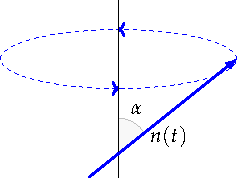
\includegraphics[]{Images/fig-spinprecessberry.pdf}
    \caption{We consider an electron under the influence of a precessing magnetic field, which is at angle $\alpha$ to the z-axis. The polarization of the eigenspinor is also seen to precess in time.}
    \label{fig-spinprecessberry}
\end{figure}
The eigenspinor corresponding to the Hamiltonian is:
\begin{equation}
    \psi = \m{\cos\frac{\alpha}{2} \\ \sin\frac{\alpha}{2}e^{i\omega t}}
\end{equation}
which we observe is just (of course) the eigenspinor of $S_{\hat{\v{n}}}$, the spin operator in the direction $\hat{\v{n}}$ (which here is the direction of the magnetic field). The time derivative is then:
\begin{equation}
    \dpd{\psi}{t} = \m{0\\ i \omega \sin \frac{\alpha}{2}e^{i\omega t}}
\end{equation}
and so:
\begin{equation}
    \braket{\psi}{\dpd{\psi}{t}} = i\omega \sin^2\frac{\alpha}{2}
\end{equation}
So then the geometric phase at time $t$ is:
\begin{equation}
    \gamma_n(t) = \int_0^t \braket{\psi}{\dpd{\psi}{t'}}dt' = -\omega \sin^2\frac{\alpha}{t}t
\end{equation}
so after one period $t = T = \frac{2\pi}{\omega}$ when the B-field returns to its original position at time $0$:
\begin{equation}
    \gamma_n(T) = -2\pi\sin^2\frac{\alpha}{2} = \pi(\cos\alpha - 1)
\end{equation}
where we use $\sin^2\frac{\alpha}{2} = \frac{1 -\cos\alpha}{2}$ in the last equality. We note two results here; first, there is a non-zero phase accrued when the system returns to its original configuration. Second, this phase does not depend at all on the speed of the time-dependent Hamiltonian (there is no dependence on $\omega$).

\subsection{N-Dimensional Configuation Space}
Consider now $N$-dimensional configuration space, where $N = (R_1, \ldots R_N)$. We then see by the chain rule that:
\begin{equation}
    \dpd{\psi_n}{t} = \sum_i \dpd{\psi_n}{R_i}\dpd{R_i}{t} = \nabla_R \psi_n \dpd{\v{R}}{t}
\end{equation}
So computing the geometrical phase at time t:
\begin{equation}
    \gamma_n(t) = i\int_0^t \braket{\psi_n}{\dpd{\psi_n(t')}{t'}}dt' = i\int_{\v{R}_i}^{\v{R}_f} \braket{\psi_n}{\nabla \psi_n}d\v{R}
\end{equation}
If the Hamiltonian returns to its original form after time $T$, we can write the net geometric phase change as a loop integral:
\begin{equation}
    \gamma(T) = i\oint \braket{\psi_n}{\nabla_\v{R}\psi_n} \cdot d\v{R}
\end{equation}
which is our general formula for \emph{Berry's phase}.